\documentclass{beamer}
\mode<presentation>
\usepackage{amsmath}
\usepackage{amssymb}
\usepackage{adjustbox}
\usepackage{subcaption}
\usepackage{enumitem}
\usepackage{multicol}
\usepackage{mathtools}
\usepackage{listings}
\usepackage{url}
\def\UrlBreaks{\do\/\do-}
\usetheme{Boadilla}
\usecolortheme{lily}
\setbeamertemplate{footline}
{
  \leavevmode%
  \hbox{%
  \begin{beamercolorbox}[wd=\paperwidth,ht=2.25ex,dp=1ex,right]{author in head/foot}%
    \insertframenumber{} / \inserttotalframenumber\hspace*{2ex} 
  \end{beamercolorbox}}%
  \vskip0pt%
}

\providecommand{\nCr}[2]{\,^{#1}C_{#2}} % nCr
\providecommand{\nPr}[2]{\,^{#1}P_{#2}} % nPr
\providecommand{\mbf}{\mathbf}
\providecommand{\pr}[1]{\ensuremath{\Pr\left(#1\right)}}
\providecommand{\qfunc}[1]{\ensuremath{Q\left(#1\right)}}
\providecommand{\sbrak}[1]{\ensuremath{{}\left[#1\right]}}
\providecommand{\lsbrak}[1]{\ensuremath{{}\left[#1\right.}}
\providecommand{\rsbrak}[1]{\ensuremath{{}\left.#1\right]}}
\providecommand{\brak}[1]{\ensuremath{\left(#1\right)}}
\providecommand{\lbrak}[1]{\ensuremath{\left(#1\right.}}
\providecommand{\rbrak}[1]{\ensuremath{\left.#1\right)}}
\providecommand{\cbrak}[1]{\ensuremath{\left\{#1\right\}}}
\providecommand{\lcbrak}[1]{\ensuremath{\left\{#1\right.}}
\providecommand{\rcbrak}[1]{\ensuremath{\left.#1\right\}}}
\theoremstyle{remark}
\newtheorem{rem}{Remark}
\newcommand{\sgn}{\mathop{\mathrm{sgn}}}
\providecommand{\abs}[1]{$\left\vert#1\right\vert$}
\providecommand{\res}[1]{\Res\displaylimits_{#1}} 
\providecommand{\norm}[1]{\lVert#1\rVert}
\providecommand{\mtx}[1]{\mathbf{#1}}
\providecommand{\mean}[1]{$E\left[ #1 \right]$}
\providecommand{\fourier}{\overset{\mathcal{F}}{ \rightleftharpoons}}
%\providecommand{\hilbert}{\overset{\mathcal{H}}{ \rightleftharpoons}}
\providecommand{\system}{\overset{\mathcal{H}}{ \longleftrightarrow}}
	%\newcommand{\solution}[2]{\textbf{Solution:}{#1}}
%\newcommand{\solution}{\noindent \textbf{Solution: }}
\providecommand{\dec}[2]{\ensuremath{\overset{#1}{\underset{#2}{\gtrless}}}}
\newcommand{\myvec}[1]{\ensuremath{\begin{pmatrix}#1\end{pmatrix}}}
\let\vec\mathbf

\lstset{
%language=C,
frame=single, 
breaklines=true,
columns=fullflexible
}

\numberwithin{equation}{section}

\lstset{
  language=Python,
  basicstyle=\ttfamily\small,
  keywordstyle=\color{blue},
  stringstyle=\color{orange},
  numbers=left,
  numberstyle=\tiny\color{gray},
  breaklines=true,
  showstringspaces=false
}

\title{Problem 1.5.13}
\author{EE25BTECH11025-Vishwambhar}

\date{\today} 
\begin{document}

\begin{frame}
\titlepage
\end{frame}

\section*{Outline}
\begin{frame}
\tableofcontents
\end{frame}
\section{Problem}
\begin{frame}
\frametitle{Problem Statement}
Find the ratio in which the $Y$ axis divides the line segment joining the points $\vec{A}\brak{-1,-4}$ and $\vec{B}\brak{5,-6}$. Also find the coordinates of the point of intersection.\\
\end{frame}

\section{Solution}

\subsection{Variables used}
\begin{frame}
\frametitle{Variables used}
\begin{tabular}[12pt]{|c|c|}
\hline
\textbf{Variable}&\textbf{characteristic}\\
\hline
$\vec{C}$&point of intersection of the line segment and y-axis\\
\hline
$x$&x-coordinate of the point $\vec{C}$\\
\hline
$y$&y-coordinate of point $\vec{C}$\\
\hline
$m$&Slope of line segment joining $\vec{A}$ and $\vec{B}$\\
\hline
\end{tabular}
\end{frame}

\subsection{Slope$\brak{m}$}
\begin{frame}
\frametitle{Slope$\brak{m}$}
Slope of line segment joining $\vec{A}$ and $\vec{B}$:\\
\begin{align}
m=\frac{\brak{-6}-\brak{-4}}{5-\brak{-1}}\\
m=\brak{\frac{-1}{3}}
\end{align}
\end{frame}

\subsection{Obtaining Point}
\begin{frame}
\frametitle{Obtaining Point}
The point of intersection of the given line segment and the $Y$-axis is:\\
\begin{align}
\myvec{1&3\\1&0}\myvec{x\\y}=\myvec{-13\\0}\\
\myvec{x\\y}=\myvec{0\\\brak{\frac{-13}{3}}}
\end{align}
\end{frame}

\subsection{Ratio}
\begin{frame}
\frametitle{Ratio}
The ratio in which the $Y$-axis divides the given line segment is:\\
\begin{align}
    {\frac{AC}{CB}}=\frac{1}{5}
\end{align}
\end{frame}

\subsection{Plot}
\begin{frame}[fragile]
\frametitle{Plot}
\begin{figure}[h!]
   \centering
   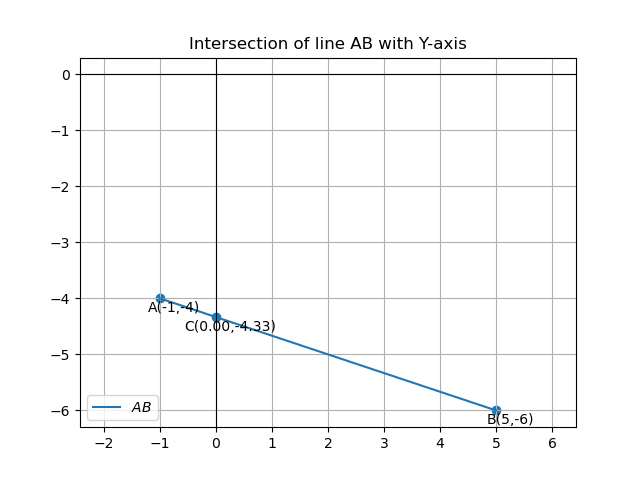
\includegraphics[width=0.9\linewidth]{figs/plot.png}
	\caption{Area Enclosed by parabola and line. }
   \label{stemplot}
\end{figure}
\end{frame}

\section{C Code}
\begin{frame}[fragile]
\frametitle{C Code for assigning matrices}
\begin{lstlisting}[language=C]
#include <stdio.h>
#include <math.h>
#include <stdlib.h>
#include "libs/matfun.h"
#include "libs/geofun.h"

int main(){
	int n=2;
	double **A, **b, **A_inv, **x;

	A=createMat(n,n);
	b=createMat(n,1);
	x=createMat(n,1);


	A[0][0]=1; A[0][1]=1;
	A[1][0]=3; A[1][1]=0;

	b[0][0]= -13;
	b[1][0]= 0;
 
    \end{lstlisting}
\end{frame}
\begin{frame}[fragile]
\frametitle{C Code for finding inverse of a matrix and also the point of intersection} 
\begin{lstlisting}[language=C]
  	A_inv = Matinv(A,n);
    x=Matmul(A_inv,b,n,n,1);
    printf("Solution of Ax=b:\n");
	for(int i=0;i<n;i++){
		printf("x[%d]=%.2f\n", i+1, x[i][0]);
	}
 \end{lstlisting}
\end{frame}

\begin{frame}[fragile]
\frametitle{C Code for storing values in a file}
\begin{lstlisting}[language=C]
FILE *file=fopen("values.dat", "w");
	if(file==NULL){
		printf("Error opening file!\n");
		return 1;
	}
	fprintf(file, "The point of intersection of the line segment and the Y-axis is:\n");
		fprintf(file, "x-coordinate    y-coordinate\n");
		fprintf(file, "   %.2f              %.2f",x[0][0], x[1][0]);
	fclose(file);
	printf("Results have been written to values.dat\n");
	freeMat(A,n);
	freeMat(b,n);
	freeMat(A_inv,n);
	freeMat(x,n);
        return 0;
}
\end{lstlisting}
\end{frame}

\section{Python Code}
\begin{frame}[fragile]
\frametitle{Python Code for Plotting}
\begin{lstlisting}[language=Python]
import sys
import numpy as np
import matplotlib.pyplot as plt

# Add your workspace path (adjust if needed)
sys.path.insert(0, '/home/ganachari-vishwmabhar/Downloads/codes/CoordGeo')

# Local imports
from line.funcs import line_gen

# Read intersection point from values.dat (skip first two rows if it has header)
data = np.loadtxt("values.dat", skiprows=2)
xc, yc = data[0], data[1]
C = np.array([xc, yc]).reshape(-1, 1)
\end{lstlisting}
\end{frame}

\begin{frame}[fragile]
\frametitle{Python Code for Plotting}
\begin{lstlisting}[language=Python]
# Given points
A = np.array([-1, -4]).reshape(-1, 1)
B = np.array([5, -6]).reshape(-1, 1)

# Generate line AB using helper function
x_AB = line_gen(A, B)

# ---- Plotting ----
plt.plot(x_AB[0, :], x_AB[1, :], label='$AB$')

# Collect points
tri_coords = np.block([A, B, C])
plt.scatter(tri_coords[0, :], tri_coords[1, :])

# Labels
vert_labels = ['A(-1,-4)', 'B(5,-6)', f'C({xc:.2f},{yc:.2f})']
\end{lstlisting}
\end{frame}

\begin{frame}[fragile]
\frametitle{Python Code for Plotting}
\begin{lstlisting}[language=Python]
for i, txt in enumerate(vert_labels):
    x, y = tri_coords[:, i]
    plt.annotate(txt, (x, y),
                 textcoords="offset points",
                 xytext=(10, -10),
                 ha='center')

# Axes styling
plt.axhline(0, color='black', linewidth=0.8)
plt.axvline(0, color='black', linewidth=0.8)
plt.grid(True)
plt.axis('equal')
plt.legend()
plt.title("Intersection of line AB with Y-axis")

# Save & Show
plt.savefig('../figs/fig1.png')
plt.show()
\end{lstlisting}
\end{frame}


\end{document}